% Options for packages loaded elsewhere
\PassOptionsToPackage{unicode}{hyperref}
\PassOptionsToPackage{hyphens}{url}
%
\documentclass[
  ignorenonframetext,
  aspectratio=169]{beamer}
\usepackage{pgfpages}
\setbeamertemplate{caption}[numbered]
\setbeamertemplate{caption label separator}{: }
\setbeamercolor{caption name}{fg=normal text.fg}
\beamertemplatenavigationsymbolsempty
% Prevent slide breaks in the middle of a paragraph
\widowpenalties 1 10000
\raggedbottom
\setbeamertemplate{part page}{
  \centering
  \begin{beamercolorbox}[sep=16pt,center]{part title}
    \usebeamerfont{part title}\insertpart\par
  \end{beamercolorbox}
}
\setbeamertemplate{section page}{
  \centering
  \begin{beamercolorbox}[sep=12pt,center]{part title}
    \usebeamerfont{section title}\insertsection\par
  \end{beamercolorbox}
}
\setbeamertemplate{subsection page}{
  \centering
  \begin{beamercolorbox}[sep=8pt,center]{part title}
    \usebeamerfont{subsection title}\insertsubsection\par
  \end{beamercolorbox}
}
\AtBeginPart{
  \frame{\partpage}
}
\AtBeginSection{
  \ifbibliography
  \else
    \frame{\sectionpage}
  \fi
}
\AtBeginSubsection{
  \frame{\subsectionpage}
}
\usepackage{amsmath,amssymb}
\usepackage{lmodern}
\usepackage{ifxetex,ifluatex}
\ifnum 0\ifxetex 1\fi\ifluatex 1\fi=0 % if pdftex
  \usepackage[T1]{fontenc}
  \usepackage[utf8]{inputenc}
  \usepackage{textcomp} % provide euro and other symbols
\else % if luatex or xetex
  \usepackage{unicode-math}
  \defaultfontfeatures{Scale=MatchLowercase}
  \defaultfontfeatures[\rmfamily]{Ligatures=TeX,Scale=1}
\fi
% Use upquote if available, for straight quotes in verbatim environments
\IfFileExists{upquote.sty}{\usepackage{upquote}}{}
\IfFileExists{microtype.sty}{% use microtype if available
  \usepackage[]{microtype}
  \UseMicrotypeSet[protrusion]{basicmath} % disable protrusion for tt fonts
}{}
\makeatletter
\@ifundefined{KOMAClassName}{% if non-KOMA class
  \IfFileExists{parskip.sty}{%
    \usepackage{parskip}
  }{% else
    \setlength{\parindent}{0pt}
    \setlength{\parskip}{6pt plus 2pt minus 1pt}}
}{% if KOMA class
  \KOMAoptions{parskip=half}}
\makeatother
\usepackage{xcolor}
\IfFileExists{xurl.sty}{\usepackage{xurl}}{} % add URL line breaks if available
\IfFileExists{bookmark.sty}{\usepackage{bookmark}}{\usepackage{hyperref}}
\hypersetup{
  pdftitle={Differences between regression models and SIMMs},
  pdfauthor={Andrew Parnell   },
  hidelinks,
  pdfcreator={LaTeX via pandoc}}
\urlstyle{same} % disable monospaced font for URLs
\newif\ifbibliography
\usepackage{color}
\usepackage{fancyvrb}
\newcommand{\VerbBar}{|}
\newcommand{\VERB}{\Verb[commandchars=\\\{\}]}
\DefineVerbatimEnvironment{Highlighting}{Verbatim}{commandchars=\\\{\}}
% Add ',fontsize=\small' for more characters per line
\usepackage{framed}
\definecolor{shadecolor}{RGB}{248,248,248}
\newenvironment{Shaded}{\begin{snugshade}}{\end{snugshade}}
\newcommand{\AlertTok}[1]{\textcolor[rgb]{0.94,0.16,0.16}{#1}}
\newcommand{\AnnotationTok}[1]{\textcolor[rgb]{0.56,0.35,0.01}{\textbf{\textit{#1}}}}
\newcommand{\AttributeTok}[1]{\textcolor[rgb]{0.77,0.63,0.00}{#1}}
\newcommand{\BaseNTok}[1]{\textcolor[rgb]{0.00,0.00,0.81}{#1}}
\newcommand{\BuiltInTok}[1]{#1}
\newcommand{\CharTok}[1]{\textcolor[rgb]{0.31,0.60,0.02}{#1}}
\newcommand{\CommentTok}[1]{\textcolor[rgb]{0.56,0.35,0.01}{\textit{#1}}}
\newcommand{\CommentVarTok}[1]{\textcolor[rgb]{0.56,0.35,0.01}{\textbf{\textit{#1}}}}
\newcommand{\ConstantTok}[1]{\textcolor[rgb]{0.00,0.00,0.00}{#1}}
\newcommand{\ControlFlowTok}[1]{\textcolor[rgb]{0.13,0.29,0.53}{\textbf{#1}}}
\newcommand{\DataTypeTok}[1]{\textcolor[rgb]{0.13,0.29,0.53}{#1}}
\newcommand{\DecValTok}[1]{\textcolor[rgb]{0.00,0.00,0.81}{#1}}
\newcommand{\DocumentationTok}[1]{\textcolor[rgb]{0.56,0.35,0.01}{\textbf{\textit{#1}}}}
\newcommand{\ErrorTok}[1]{\textcolor[rgb]{0.64,0.00,0.00}{\textbf{#1}}}
\newcommand{\ExtensionTok}[1]{#1}
\newcommand{\FloatTok}[1]{\textcolor[rgb]{0.00,0.00,0.81}{#1}}
\newcommand{\FunctionTok}[1]{\textcolor[rgb]{0.00,0.00,0.00}{#1}}
\newcommand{\ImportTok}[1]{#1}
\newcommand{\InformationTok}[1]{\textcolor[rgb]{0.56,0.35,0.01}{\textbf{\textit{#1}}}}
\newcommand{\KeywordTok}[1]{\textcolor[rgb]{0.13,0.29,0.53}{\textbf{#1}}}
\newcommand{\NormalTok}[1]{#1}
\newcommand{\OperatorTok}[1]{\textcolor[rgb]{0.81,0.36,0.00}{\textbf{#1}}}
\newcommand{\OtherTok}[1]{\textcolor[rgb]{0.56,0.35,0.01}{#1}}
\newcommand{\PreprocessorTok}[1]{\textcolor[rgb]{0.56,0.35,0.01}{\textit{#1}}}
\newcommand{\RegionMarkerTok}[1]{#1}
\newcommand{\SpecialCharTok}[1]{\textcolor[rgb]{0.00,0.00,0.00}{#1}}
\newcommand{\SpecialStringTok}[1]{\textcolor[rgb]{0.31,0.60,0.02}{#1}}
\newcommand{\StringTok}[1]{\textcolor[rgb]{0.31,0.60,0.02}{#1}}
\newcommand{\VariableTok}[1]{\textcolor[rgb]{0.00,0.00,0.00}{#1}}
\newcommand{\VerbatimStringTok}[1]{\textcolor[rgb]{0.31,0.60,0.02}{#1}}
\newcommand{\WarningTok}[1]{\textcolor[rgb]{0.56,0.35,0.01}{\textbf{\textit{#1}}}}
\usepackage{graphicx}
\makeatletter
\def\maxwidth{\ifdim\Gin@nat@width>\linewidth\linewidth\else\Gin@nat@width\fi}
\def\maxheight{\ifdim\Gin@nat@height>\textheight\textheight\else\Gin@nat@height\fi}
\makeatother
% Scale images if necessary, so that they will not overflow the page
% margins by default, and it is still possible to overwrite the defaults
% using explicit options in \includegraphics[width, height, ...]{}
\setkeys{Gin}{width=\maxwidth,height=\maxheight,keepaspectratio}
% Set default figure placement to htbp
\makeatletter
\def\fps@figure{htbp}
\makeatother
\setlength{\emergencystretch}{3em} % prevent overfull lines
\providecommand{\tightlist}{%
  \setlength{\itemsep}{0pt}\setlength{\parskip}{0pt}}
\setcounter{secnumdepth}{-\maxdimen} % remove section numbering
\usepackage{graphicx}
\usepackage{amsmath,amsfonts,amssymb,amsthm,amscd, mathrsfs}
\setbeamertemplate{navigation symbols}{} %%removes bottom line
\setbeamertemplate{footline}[frame number]
\ifluatex
  \usepackage{selnolig}  % disable illegal ligatures
\fi

\title{Differences between regression models and SIMMs}
\author{Andrew Parnell \newline \texttt{andrew.parnell@mu.ie}
\newline \vspace{1cm}
\newline 
\includegraphics[width=3cm]{../maynooth_uni_logo.jpg}}
\date{}

\begin{document}
\frame{\titlepage}

\begin{frame}{Learning outcomes}
\protect\hypertarget{learning-outcomes}{}
\begin{itemize}
\tightlist
\item
  Be able to describe the differences and similarities between a
  regression model and a SIMM
\item
  Understand the likelihood and prior distribution in a basic SIMM
\item
  Know how to check convergence and model performance in a Bayesian
  model
\end{itemize}
\end{frame}

\begin{frame}{Revision: linear regression}
\protect\hypertarget{revision-linear-regression}{}
\begin{itemize}
\tightlist
\item
  In many statistical problems we have a \emph{response variable}
  \(y_i\) observed on individuals \(i=1,\ldots,N\)
\item
  We also have an \emph{explanatory variable} \(x_i\) from which we want
  to predict \(y_i\)
\item
  For example, \(y_i\) could be the weight of an animal, and \(x_i\)
  could be the proportion of a certain food source in its diet
\end{itemize}

The usual linear regression model is written as:
\[y_i = \alpha + \beta x_i + \epsilon_i\] where
\(\epsilon_i \sim N(0,\sigma^2)\). Another way of writing this model is:
\[y_i \sim N(\alpha + \beta x_i, \sigma^2)\]
\end{frame}

\begin{frame}[fragile]{Example: simple data}
\protect\hypertarget{example-simple-data}{}
\small

\begin{Shaded}
\begin{Highlighting}[]
\NormalTok{x}\OtherTok{=}\FunctionTok{c}\NormalTok{(}\FloatTok{18.07}\NormalTok{, }\FloatTok{52.59}\NormalTok{, }\FloatTok{54.93}\NormalTok{, }\FloatTok{79.31}\NormalTok{, }\FloatTok{89.58}\NormalTok{)}
\NormalTok{y}\OtherTok{=}\FunctionTok{c}\NormalTok{(}\FloatTok{7.89}\NormalTok{, }\FloatTok{12.41}\NormalTok{, }\FloatTok{13.34}\NormalTok{, }\FloatTok{19.3}\NormalTok{, }\FloatTok{19.52}\NormalTok{)}
\FunctionTok{plot}\NormalTok{(x,y,}
     \AttributeTok{xlab=}\StringTok{\textquotesingle{}Percentage of food source in diet (x)\textquotesingle{}}\NormalTok{,}
     \AttributeTok{ylab=}\StringTok{\textquotesingle{}Weight (y)\textquotesingle{}}\NormalTok{,}
     \AttributeTok{las=}\DecValTok{1}\NormalTok{)}
\FunctionTok{abline}\NormalTok{(}\AttributeTok{a=}\FloatTok{4.17}\NormalTok{,}\AttributeTok{b=}\FloatTok{0.18}\NormalTok{,}\AttributeTok{col=}\StringTok{\textquotesingle{}red\textquotesingle{}}\NormalTok{)}
\end{Highlighting}
\end{Shaded}

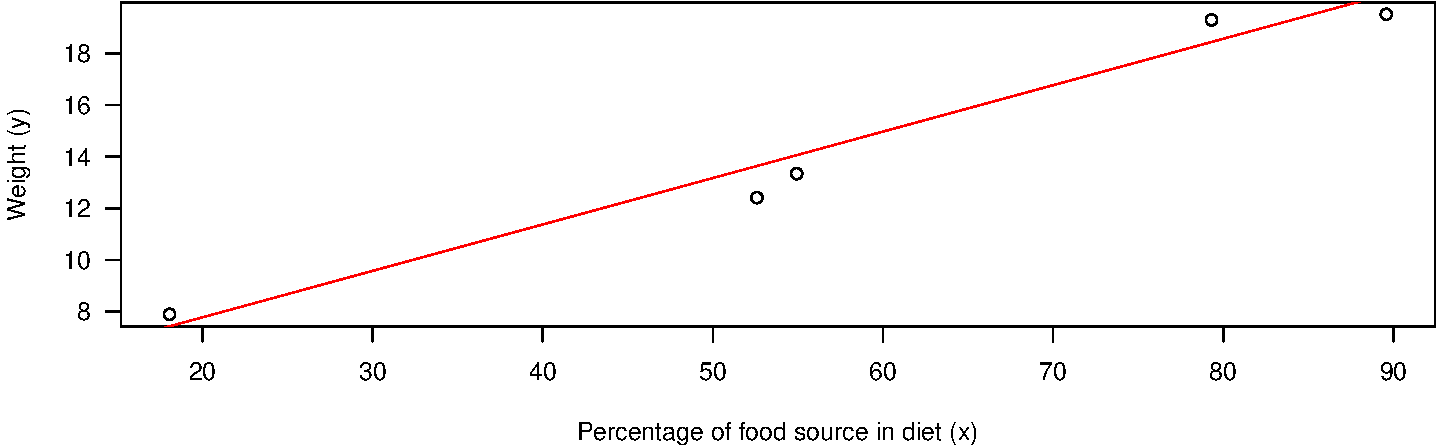
\includegraphics{reg_and_simms_files/figure-beamer/unnamed-chunk-1-1.pdf}
\end{frame}

\begin{frame}[fragile]{Running a linear regression in JAGS}
\protect\hypertarget{running-a-linear-regression-in-jags}{}
\begin{Shaded}
\begin{Highlighting}[]
\NormalTok{model\_code }\OtherTok{=}\StringTok{\textquotesingle{}}
\StringTok{model \{}
\StringTok{  for(i in 1:N) \{ }
\StringTok{    y[i] \textasciitilde{} dnorm(alpha + beta*x[i],sigma\^{}{-}2) }
\StringTok{  \}}
\StringTok{  alpha \textasciitilde{} dnorm(0,100\^{}{-}2) \# Note: vague priors}
\StringTok{  beta \textasciitilde{} dnorm(0,100\^{}{-}2)}
\StringTok{  sigma \textasciitilde{} dunif(0,100)}
\StringTok{\}}
\StringTok{\textquotesingle{}}
\NormalTok{data}\OtherTok{=}\FunctionTok{list}\NormalTok{(}\AttributeTok{x=}\FunctionTok{c}\NormalTok{(}\FloatTok{18.07}\NormalTok{, }\FloatTok{52.59}\NormalTok{, }\FloatTok{54.93}\NormalTok{, }\FloatTok{79.31}\NormalTok{, }\FloatTok{89.58}\NormalTok{),}
          \AttributeTok{y=}\FunctionTok{c}\NormalTok{(}\FloatTok{7.89}\NormalTok{, }\FloatTok{12.41}\NormalTok{, }\FloatTok{13.34}\NormalTok{, }\FloatTok{19.3}\NormalTok{, }\FloatTok{19.52}\NormalTok{),}
          \AttributeTok{N=}\DecValTok{5}\NormalTok{)}
\NormalTok{model\_parameters }\OtherTok{=} \FunctionTok{c}\NormalTok{(}\StringTok{\textquotesingle{}alpha\textquotesingle{}}\NormalTok{, }\StringTok{\textquotesingle{}beta\textquotesingle{}}\NormalTok{, }\StringTok{\textquotesingle{}sigma\textquotesingle{}}\NormalTok{)}
\NormalTok{model\_run }\OtherTok{=} \FunctionTok{jags}\NormalTok{(}\AttributeTok{data =}\NormalTok{ data,}
                 \AttributeTok{parameters.to.save =}\NormalTok{ model\_parameters,}
                 \AttributeTok{model.file =} \FunctionTok{textConnection}\NormalTok{(model\_code))}
\end{Highlighting}
\end{Shaded}

\begin{verbatim}
## module glm loaded
\end{verbatim}
\end{frame}

\begin{frame}[fragile]{Output from linear regression}
\protect\hypertarget{output-from-linear-regression}{}
\small

\begin{Shaded}
\begin{Highlighting}[]
\FunctionTok{par}\NormalTok{(}\AttributeTok{mfrow=}\FunctionTok{c}\NormalTok{(}\DecValTok{1}\NormalTok{,}\DecValTok{2}\NormalTok{))}
\NormalTok{post }\OtherTok{=}\NormalTok{ model\_run}\SpecialCharTok{$}\NormalTok{BUGSoutput}\SpecialCharTok{$}\NormalTok{sims.list}
\FunctionTok{plot}\NormalTok{(}\FunctionTok{density}\NormalTok{(post}\SpecialCharTok{$}\NormalTok{alpha),}\AttributeTok{main=}\StringTok{\textquotesingle{}Posterior for alpha\textquotesingle{}}\NormalTok{)}
\FunctionTok{plot}\NormalTok{(}\FunctionTok{density}\NormalTok{(post}\SpecialCharTok{$}\NormalTok{beta),}\AttributeTok{main=}\StringTok{\textquotesingle{}Posterior for beta\textquotesingle{}}\NormalTok{)}
\end{Highlighting}
\end{Shaded}

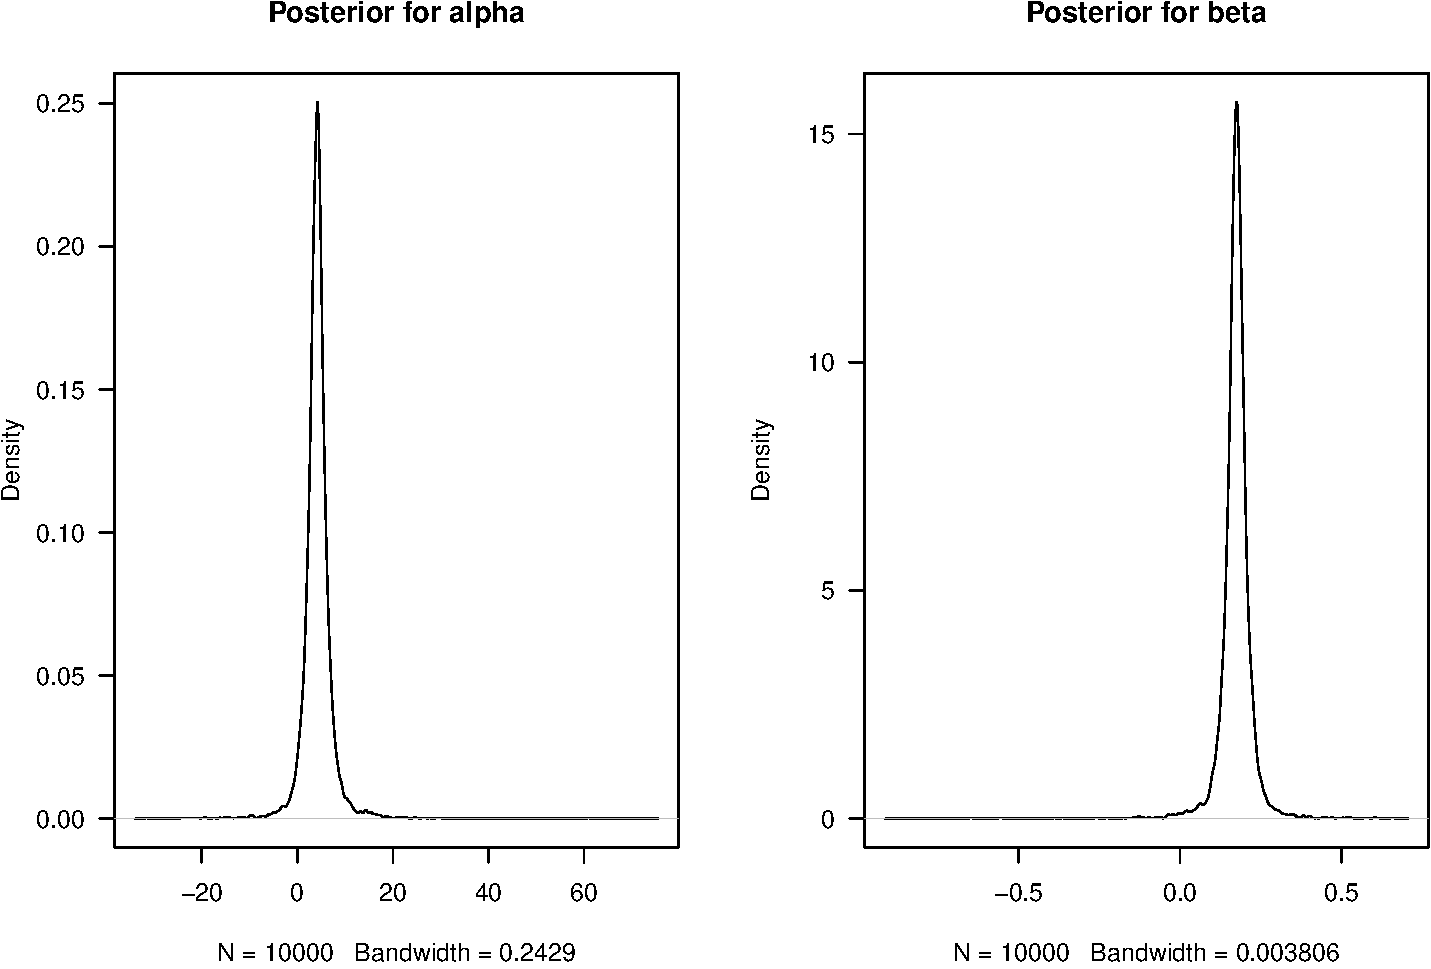
\includegraphics{reg_and_simms_files/figure-beamer/unnamed-chunk-4-1.pdf}
\end{frame}

\begin{frame}[fragile]{More output from linear regression}
\protect\hypertarget{more-output-from-linear-regression}{}
\small

\begin{Shaded}
\begin{Highlighting}[]
\FunctionTok{print}\NormalTok{(model\_run)}
\end{Highlighting}
\end{Shaded}

\begin{verbatim}
## Inference for Bugs model at "4", fit using jags,
##  3 chains, each with 2000 iterations (first 1000 discarded)
##  n.sims = 3000 iterations saved
##          mu.vect sd.vect   2.5%    25%    50%    75%  97.5%  Rhat n.eff
## alpha      4.041   3.121 -2.276  2.905  4.113  5.267 10.088 1.013  3000
## beta       0.177   0.049  0.080  0.158  0.176  0.195  0.277 1.010  2400
## sigma      2.052   1.603  0.639  1.057  1.502  2.402  6.991 1.006   420
## deviance  18.288   5.083 12.244 14.398 16.874 20.939 31.139 1.006   350
## 
## For each parameter, n.eff is a crude measure of effective sample size,
## and Rhat is the potential scale reduction factor (at convergence, Rhat=1).
## 
## DIC info (using the rule, pD = var(deviance)/2)
## pD = 12.9 and DIC = 31.2
## DIC is an estimate of expected predictive error (lower deviance is better).
\end{verbatim}
\end{frame}

\begin{frame}{How do we choose a likelihood and a prior for this
situation?}
\protect\hypertarget{how-do-we-choose-a-likelihood-and-a-prior-for-this-situation}{}
\begin{itemize}
\tightlist
\item
  When we're in a standard linear regression situation the likelihood is
  always a normal distribution. When we use other likelihoods we're
  running a \emph{generalised linear model}
\item
  The prior for the intercept (\(\alpha\)) and slope (\(\beta\)) might
  come from previous experiments, or in this case are set as vague.
  Similarly for the residual standard deviation
\item
  Sometimes \emph{re-parameterising} the model will help with setting
  the priors. For example, it might be easier to re-write the model as
  \(y_i = \alpha + \beta (x_i - \bar{x}) + \epsilon_i\). Now the
  parameter \(\alpha\) represents the mean value of \(y\) at the mean
  value of \(x\) (denoted \(\bar{x}\)). This might be easier to put a
  prior distribution on
\end{itemize}
\end{frame}

\begin{frame}{Example 2: a generalised linear model situation,
e.g.~Logistic regression}
\protect\hypertarget{example-2-a-generalised-linear-model-situation-e.g.-logistic-regression}{}
\begin{itemize}
\tightlist
\item
  Suppose now that rather than observing \(y\) as the weight of the
  animal, we have observed \(y\) as whether or not the animal was male
  (\(y_i=1\)) or female (\(y_i=0\))
\item
  The goal of the model is now to estimate the relationship between
  dietary proportion and the probability of being male.
\item
  When the response variable is binary we use a GLM called
  \emph{logistic regression}. We can write this new model as:
  \[ y_i \sim Bin(1,p_i),\; logit(p_i) = \alpha + \beta x_i\] where
  \(logit(p) = \log \left( \frac{p}{1-p} \right)\). Note that \(p_i\)
  directly measures the probability of each individual being male and
  has to lie between 0 and 1
\end{itemize}
\end{frame}

\begin{frame}[fragile]{Example 2 in JAGS}
\protect\hypertarget{example-2-in-jags}{}
\small

Note: this isn't a great model as the data set is very small

\begin{Shaded}
\begin{Highlighting}[]
\NormalTok{model\_code }\OtherTok{=}\StringTok{\textquotesingle{}}
\StringTok{model \{}
\StringTok{  for(i in 1:N) \{ }
\StringTok{    y[i] \textasciitilde{} dbin(p[i],1) }
\StringTok{    logit(p[i]) \textless{}{-} alpha + beta*x[i]}
\StringTok{  \}}
\StringTok{  alpha \textasciitilde{} dnorm(0,4\^{}{-}2)}
\StringTok{  beta \textasciitilde{} dnorm(0,4\^{}{-}2)}
\StringTok{\}}
\StringTok{\textquotesingle{}}
\NormalTok{data}\OtherTok{=}\FunctionTok{list}\NormalTok{(}\AttributeTok{x=}\FunctionTok{c}\NormalTok{(}\FloatTok{18.07}\NormalTok{, }\FloatTok{52.59}\NormalTok{, }\FloatTok{54.93}\NormalTok{, }\FloatTok{79.31}\NormalTok{, }\FloatTok{89.58}\NormalTok{),}
          \AttributeTok{y=}\FunctionTok{c}\NormalTok{(}\DecValTok{0}\NormalTok{,}\DecValTok{1}\NormalTok{,}\DecValTok{0}\NormalTok{,}\DecValTok{1}\NormalTok{,}\DecValTok{1}\NormalTok{),}
          \AttributeTok{N=}\DecValTok{5}\NormalTok{)}
\NormalTok{model\_parameters }\OtherTok{=} \FunctionTok{c}\NormalTok{(}\StringTok{\textquotesingle{}alpha\textquotesingle{}}\NormalTok{, }\StringTok{\textquotesingle{}beta\textquotesingle{}}\NormalTok{)}
\NormalTok{model\_run }\OtherTok{=} \FunctionTok{jags}\NormalTok{(}\AttributeTok{data =}\NormalTok{ data,}
                 \AttributeTok{parameters.to.save =}\NormalTok{ model\_parameters,}
                 \AttributeTok{model.file =} \FunctionTok{textConnection}\NormalTok{(model\_code))}
\end{Highlighting}
\end{Shaded}

\begin{verbatim}
## Compiling model graph
##    Resolving undeclared variables
##    Allocating nodes
## Graph information:
##    Observed stochastic nodes: 5
##    Unobserved stochastic nodes: 2
##    Total graph size: 34
## 
## Initializing model
\end{verbatim}
\end{frame}

\begin{frame}[fragile]{Output}
\protect\hypertarget{output}{}
\begin{Shaded}
\begin{Highlighting}[]
\FunctionTok{plot}\NormalTok{(model\_run)}
\end{Highlighting}
\end{Shaded}

\includegraphics{reg_and_simms_files/figure-beamer/unnamed-chunk-7-1.pdf}
\end{frame}

\begin{frame}{Moving on to SIMMs - what do the data look like?}
\protect\hypertarget{moving-on-to-simms---what-do-the-data-look-like}{}
\begin{itemize}
\tightlist
\item
  Let's start with a very simple version:

  \begin{itemize}
  \tightlist
  \item
    1 isotope
  \item
    2 food sources
  \item
    9 consumers
  \item
    No other complications
  \end{itemize}
\item
  We'll use some of the Geese data that was originanlly from the SIAR
  package but is now bundled in SIBER
\end{itemize}
\end{frame}

\begin{frame}[fragile]{Plotting the data}
\protect\hypertarget{plotting-the-data}{}
\small

\begin{itemize}
\tightlist
\item
  Use the second isotope (\(\delta^{13}\)C) and the first two food
  sources (Zostera and Grass)
\item
  Create a plot:
\end{itemize}

\begin{Shaded}
\begin{Highlighting}[]
\CommentTok{\# Load in the data}
\FunctionTok{data}\NormalTok{(geese1demo); }\FunctionTok{data}\NormalTok{(sourcesdemo)}
\NormalTok{consumers }\OtherTok{=}\NormalTok{ geese1demo[,}\DecValTok{2}\NormalTok{]}
\NormalTok{sources }\OtherTok{=}\NormalTok{ sourcesdemo[}\DecValTok{1}\SpecialCharTok{:}\DecValTok{2}\NormalTok{,}\DecValTok{4}\SpecialCharTok{:}\DecValTok{5}\NormalTok{]}
\NormalTok{con\_grid }\OtherTok{=} \FunctionTok{seq}\NormalTok{(}\SpecialCharTok{{-}}\DecValTok{35}\NormalTok{,}\SpecialCharTok{{-}}\DecValTok{5}\NormalTok{,}\AttributeTok{length=}\DecValTok{100}\NormalTok{)}
\FunctionTok{plot}\NormalTok{(con\_grid,}\FunctionTok{dnorm}\NormalTok{(con\_grid,}
                    \AttributeTok{mean=}\NormalTok{sources[}\DecValTok{2}\NormalTok{,}\DecValTok{1}\NormalTok{],}\AttributeTok{sd=}\NormalTok{sources[}\DecValTok{2}\NormalTok{,}\DecValTok{2}\NormalTok{]),}
     \AttributeTok{type=}\StringTok{\textquotesingle{}l\textquotesingle{}}\NormalTok{,}\AttributeTok{col=}\StringTok{\textquotesingle{}red\textquotesingle{}}\NormalTok{,}\AttributeTok{xlab=}\StringTok{\textquotesingle{}d13C\textquotesingle{}}\NormalTok{,}\AttributeTok{ylab=}\StringTok{\textquotesingle{}Probability density\textquotesingle{}}\NormalTok{)}
\FunctionTok{lines}\NormalTok{(con\_grid,}\FunctionTok{dnorm}\NormalTok{(con\_grid}
\NormalTok{                     ,}\AttributeTok{mean=}\NormalTok{sources[}\DecValTok{1}\NormalTok{,}\DecValTok{1}\NormalTok{],}\AttributeTok{sd=}\NormalTok{sources[}\DecValTok{1}\NormalTok{,}\DecValTok{2}\NormalTok{]),}
      \AttributeTok{col=}\StringTok{\textquotesingle{}blue\textquotesingle{}}\NormalTok{)}
\FunctionTok{points}\NormalTok{(consumers,}\FunctionTok{rep}\NormalTok{(}\DecValTok{0}\NormalTok{,}\DecValTok{9}\NormalTok{))}
\FunctionTok{legend}\NormalTok{(}\StringTok{\textquotesingle{}topright\textquotesingle{}}\NormalTok{,}\AttributeTok{legend=}\FunctionTok{c}\NormalTok{(}\StringTok{\textquotesingle{}Grass\textquotesingle{}}\NormalTok{,}\StringTok{\textquotesingle{}Zostera\textquotesingle{}}\NormalTok{,}\StringTok{\textquotesingle{}Consumers\textquotesingle{}}\NormalTok{),}
       \AttributeTok{lty=}\FunctionTok{c}\NormalTok{(}\DecValTok{1}\NormalTok{,}\DecValTok{1}\NormalTok{,}\SpecialCharTok{{-}}\DecValTok{1}\NormalTok{),}\AttributeTok{pch=}\FunctionTok{c}\NormalTok{(}\SpecialCharTok{{-}}\DecValTok{1}\NormalTok{,}\SpecialCharTok{{-}}\DecValTok{1}\NormalTok{,}\DecValTok{1}\NormalTok{),}\AttributeTok{col=}\FunctionTok{c}\NormalTok{(}\StringTok{\textquotesingle{}red\textquotesingle{}}\NormalTok{,}\StringTok{\textquotesingle{}blue\textquotesingle{}}\NormalTok{,}\StringTok{\textquotesingle{}black\textquotesingle{}}\NormalTok{))}
\end{Highlighting}
\end{Shaded}
\end{frame}

\begin{frame}{A simple isospace plot}
\protect\hypertarget{a-simple-isospace-plot}{}
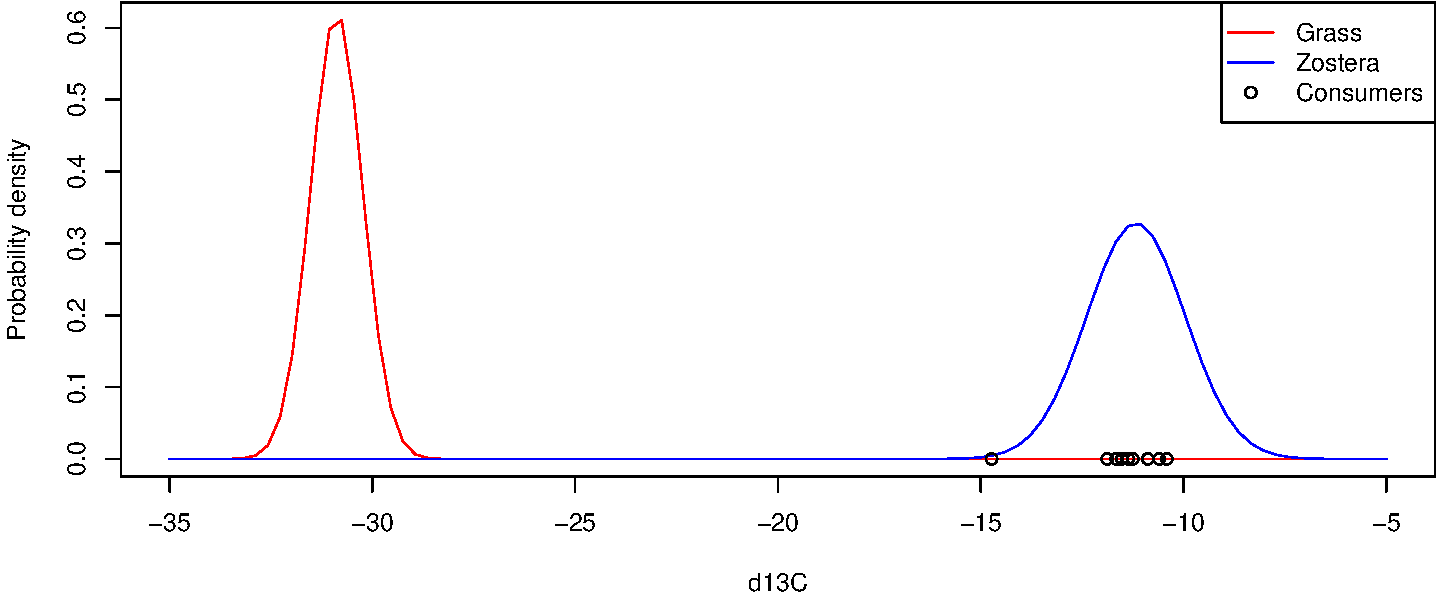
\includegraphics{reg_and_simms_files/figure-beamer/unnamed-chunk-10-1.pdf}
\end{frame}

\begin{frame}{A first model for this simple SIMM}
\protect\hypertarget{a-first-model-for-this-simple-simm}{}
\begin{itemize}
\tightlist
\item
  Let \(y_i\) be the \(\delta^{13}\)C value for individual \(i\),
  \(i=1,\ldots,9\)
\item
  Let \(s_k\) be the source value for source \(k\), \(k=1,2\)
\item
  Let \(p_k\) be the dietary proportion for source \(k\)
\end{itemize}

The likelihood can now be written as:
\[ y_i = p_1 \times s_1 + p_2 \times s_2 + \epsilon_i \;\mbox{or}\; y_i \sim N\left(\sum_{k=1}^2 p_ks_k,\sigma^2\right)\]

so just like a regression model with a slightly different mean!

\(\epsilon_i \sim N(0,\sigma^2)\) as usual, though including this term
is (strangely) controversial
\end{frame}

\begin{frame}{Prior distributions for the SIMM}
\protect\hypertarget{prior-distributions-for-the-simm}{}
\begin{itemize}
\tightlist
\item
  The parameters for this simple model are \(s_1,s_2\), \(p_1,p_2\), and
  \(\sigma\)
\item
  We have external data on the \(s_k\) values, so it makes sense to put
  a prior distribution \(s_k \sim N(\mu_{s_k},\sigma_{s_k}^2)\) on each
  of these
\item
  The dietary proportions must sum to 1, i.e.~\(p_2 = 1-p_1\) so we have
  only have 1 parameter to place a prior on. We might use
  \(p_1 \sim U(0,1)\) if no prior knowledge.
\item
  An alternative is the Beta distribution which can put more weight on
  lower or higher proportions
\item
  We usually have little information on \(\sigma\), but the isospace
  plot will usually give a rough guide to the likely range of values
\end{itemize}
\end{frame}

\begin{frame}[fragile]{A simple SIMM in JAGS}
\protect\hypertarget{a-simple-simm-in-jags}{}
\small

\begin{Shaded}
\begin{Highlighting}[]
\NormalTok{model\_code }\OtherTok{=}\StringTok{\textquotesingle{}}
\StringTok{model \{}
\StringTok{  for(i in 1:N) \{ }
\StringTok{    y[i] \textasciitilde{} dnorm(p\_1*s\_1+p\_2*s\_2,sigma\^{}{-}2) }
\StringTok{  \}}
\StringTok{  p\_1 \textasciitilde{} dunif(0,1)}
\StringTok{  p\_2 \textless{}{-} 1{-}p\_1}
\StringTok{  s\_1 \textasciitilde{} dnorm(s\_1\_mean,s\_1\_sd\^{}{-}2)}
\StringTok{  s\_2 \textasciitilde{} dnorm(s\_2\_mean,s\_2\_sd\^{}{-}2)}
\StringTok{  sigma \textasciitilde{} dunif(0,10)}
\StringTok{\}}
\StringTok{\textquotesingle{}}
\NormalTok{data}\OtherTok{=}\FunctionTok{list}\NormalTok{(}\AttributeTok{y=}\NormalTok{consumers,}\AttributeTok{s\_1\_mean=}\NormalTok{sources[}\DecValTok{1}\NormalTok{,}\DecValTok{1}\NormalTok{],}
          \AttributeTok{s\_1\_sd=}\NormalTok{sources[}\DecValTok{1}\NormalTok{,}\DecValTok{2}\NormalTok{],}
          \AttributeTok{s\_2\_mean=}\NormalTok{sources[}\DecValTok{2}\NormalTok{,}\DecValTok{1}\NormalTok{],}\AttributeTok{s\_2\_sd=}\NormalTok{sources[}\DecValTok{2}\NormalTok{,}\DecValTok{2}\NormalTok{],}
          \AttributeTok{N=}\FunctionTok{length}\NormalTok{(consumers))}
\NormalTok{model\_parameters }\OtherTok{=} \FunctionTok{c}\NormalTok{(}\StringTok{\textquotesingle{}p\_1\textquotesingle{}}\NormalTok{, }\StringTok{\textquotesingle{}p\_2\textquotesingle{}}\NormalTok{)}
\NormalTok{model\_run }\OtherTok{=} \FunctionTok{jags}\NormalTok{(}\AttributeTok{data =}\NormalTok{ data,}
                 \AttributeTok{parameters.to.save =}\NormalTok{ model\_parameters,}
                 \AttributeTok{model.file =} \FunctionTok{textConnection}\NormalTok{(model\_code))}
\end{Highlighting}
\end{Shaded}
\end{frame}

\begin{frame}[fragile]{Summarising the output}
\protect\hypertarget{summarising-the-output}{}
\small

\begin{Shaded}
\begin{Highlighting}[]
\FunctionTok{hist}\NormalTok{(model\_run}\SpecialCharTok{$}\NormalTok{BUGSoutput}\SpecialCharTok{$}\NormalTok{sims.list}\SpecialCharTok{$}\NormalTok{p\_1,}
     \AttributeTok{xlim =} \FunctionTok{c}\NormalTok{(}\DecValTok{0}\NormalTok{, }\DecValTok{1}\NormalTok{),}
     \AttributeTok{xlab=}\StringTok{\textquotesingle{}Proportion\textquotesingle{}}\NormalTok{,}
     \AttributeTok{ylab=}\StringTok{\textquotesingle{}Probability density\textquotesingle{}}\NormalTok{,}
     \AttributeTok{main=}\StringTok{\textquotesingle{}Proportion of Zostera\textquotesingle{}}\NormalTok{)}
\end{Highlighting}
\end{Shaded}

\begin{center}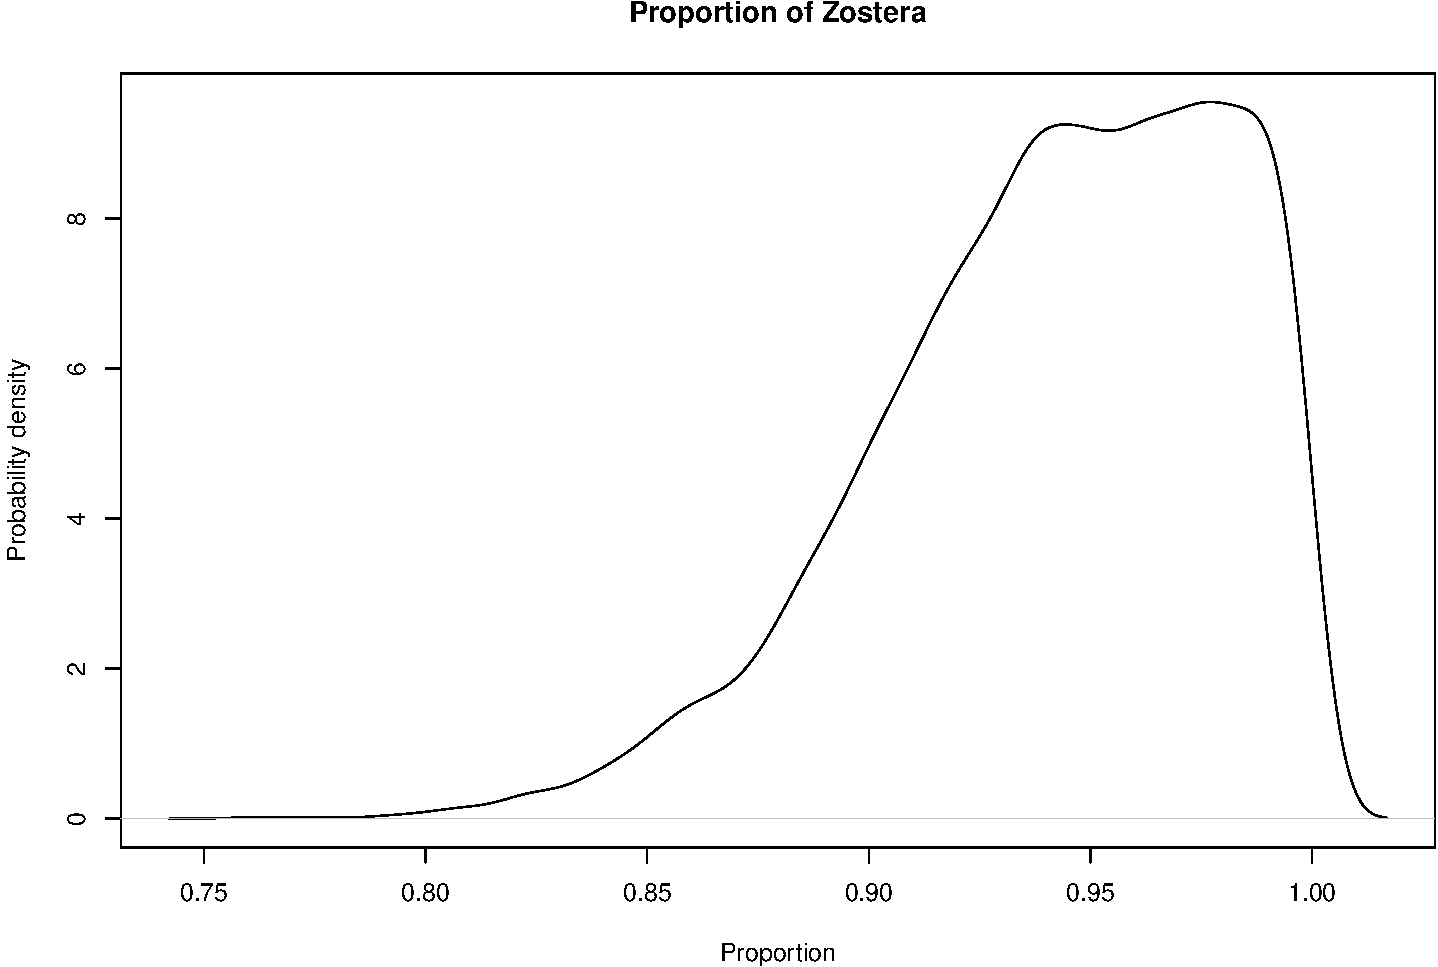
\includegraphics{reg_and_simms_files/figure-beamer/unnamed-chunk-12-1} \end{center}
\end{frame}

\begin{frame}{Model checking and convergence}
\protect\hypertarget{model-checking-and-convergence}{}
\begin{itemize}
\tightlist
\item
  How do you know whether the model fits the data well or not?
\item
  How do you know that JAGS fitted the model OK?
\item
  The model fit can be checked by running \emph{cross-validation}
  (leaving out chunks of the data and getting the model to predict the
  \(y\) values of the left out data) or \emph{posterior predictive}
  checks, amongst many other methods
\item
  The fitting performance can be evaluated via \emph{convergence
  checking}. This involves looking at the posterior samples and checking
  that the values are stable
\item
  Another question (which we will look at in a later session) is whether
  this is the `best' model for the data
\end{itemize}
\end{frame}

\begin{frame}[fragile]{Model checking}
\protect\hypertarget{model-checking}{}
\begin{itemize}
\tightlist
\item
  Adding a posterior predictive check is as simple as adding an extra
  line to the JAGS code
\end{itemize}

\begin{Shaded}
\begin{Highlighting}[]
\NormalTok{model\_code }\OtherTok{=}\StringTok{\textquotesingle{}}
\StringTok{  ...}
\StringTok{  for(i in 1:N) \{ }
\StringTok{    y[i] \textasciitilde{} dnorm(p\_1*s\_1+p\_2*s\_2,sigma\^{}{-}2) }
\StringTok{    y\_pred[i] \textasciitilde{} dnorm(p\_1*s\_1+p\_2*s\_2,sigma\^{}{-}2) }
\StringTok{  \}}
\StringTok{  ...}
\StringTok{\textquotesingle{}}
\end{Highlighting}
\end{Shaded}

\begin{itemize}
\tightlist
\item
  \texttt{y\_pred} is included as another parameter, and is thus
  estimated as part of the model.
\item
  We then have both the true \(y\) values and some estimated \(y\)
  values from the model
\end{itemize}
\end{frame}

\begin{frame}[fragile]{Model checking output}
\protect\hypertarget{model-checking-output}{}
\small

\begin{Shaded}
\begin{Highlighting}[]
\NormalTok{y\_pred\_quantiles }\OtherTok{=} \FunctionTok{apply}\NormalTok{(model\_run}\SpecialCharTok{$}\NormalTok{BUGSoutput}\SpecialCharTok{$}\NormalTok{sims.list}\SpecialCharTok{$}\NormalTok{y\_pred,}
                         \DecValTok{2}\NormalTok{,}\StringTok{\textquotesingle{}quantile\textquotesingle{}}\NormalTok{,}
                         \AttributeTok{probs=}\FunctionTok{c}\NormalTok{(}\FloatTok{0.25}\NormalTok{,}\FloatTok{0.75}\NormalTok{))}
\FunctionTok{round}\NormalTok{(}\FunctionTok{cbind}\NormalTok{(data}\SpecialCharTok{$}\NormalTok{y,}\FunctionTok{t}\NormalTok{(y\_pred\_quantiles)),}\DecValTok{2}\NormalTok{)}
\end{Highlighting}
\end{Shaded}

\begin{verbatim}
##              25%   75%
##  [1,] 10.22 9.78 10.62
##  [2,] 10.37 9.79 10.65
##  [3,] 10.44 9.80 10.62
##  [4,] 10.52 9.82 10.66
##  [5,] 10.19 9.80 10.64
##  [6,] 10.45 9.78 10.62
##  [7,]  9.91 9.79 10.64
##  [8,] 11.27 9.79 10.66
##  [9,]  9.34 9.82 10.63
\end{verbatim}

4/9 observations outside the 50\% CI. Looks to be an OK model.
\end{frame}

\begin{frame}[fragile]{Convergence checking}
\protect\hypertarget{convergence-checking}{}
\small

\begin{itemize}
\tightlist
\item
  When JAGS runs a model it creates initial guesses of the parameter
  values and then creates many consecutive samples moving away from the
  initial values towards the true posterior distribution
\item
  Mathematical theory says that the samples must eventually come from
  the posterior distribution but this may take a very long time!
\item
  Another method for ensuring convergence is to start JAGS with multiple
  different starting values and see if each model run (known as a
  \emph{chain}) converges to the same posterior distribution
\item
  You can supply initial guesses and the number of chains to JAGS when
  you run it:
\end{itemize}

\begin{Shaded}
\begin{Highlighting}[]
\NormalTok{inits }\OtherTok{=} \ControlFlowTok{function}\NormalTok{() \{}
  \FunctionTok{list}\NormalTok{(}\StringTok{\textquotesingle{}p\_1\textquotesingle{}}\OtherTok{=}\FunctionTok{runif}\NormalTok{(}\DecValTok{1}\NormalTok{),}\StringTok{\textquotesingle{}s\_1\textquotesingle{}}\OtherTok{=}\FunctionTok{rnorm}\NormalTok{(}\DecValTok{1}\NormalTok{),}\StringTok{\textquotesingle{}s\_2\textquotesingle{}}\OtherTok{=}\FunctionTok{runif}\NormalTok{(}\DecValTok{1}\NormalTok{),}
       \StringTok{\textquotesingle{}sigma\textquotesingle{}}\OtherTok{=}\FunctionTok{runif}\NormalTok{(}\DecValTok{1}\NormalTok{,}\DecValTok{0}\NormalTok{,}\DecValTok{10}\NormalTok{))}
\NormalTok{\}}
\NormalTok{...}
\end{Highlighting}
\end{Shaded}

\begin{itemize}
\tightlist
\item
  The \texttt{model\_run} created will now contain (amongst many other
  things) a list of length 3, so we can look at the different chains
  with
  e.g.~\texttt{traceplot(model\_run,\ varname\ =\ \textquotesingle{}p\_1\textquotesingle{})}
\end{itemize}
\end{frame}

\begin{frame}[fragile]{Convergence checking 2}
\protect\hypertarget{convergence-checking-2}{}
\begin{itemize}
\tightlist
\item
  You can start by plotting the output from JAGS:
\end{itemize}

\begin{Shaded}
\begin{Highlighting}[]
\FunctionTok{plot}\NormalTok{(model\_run)}
\end{Highlighting}
\end{Shaded}

\begin{center}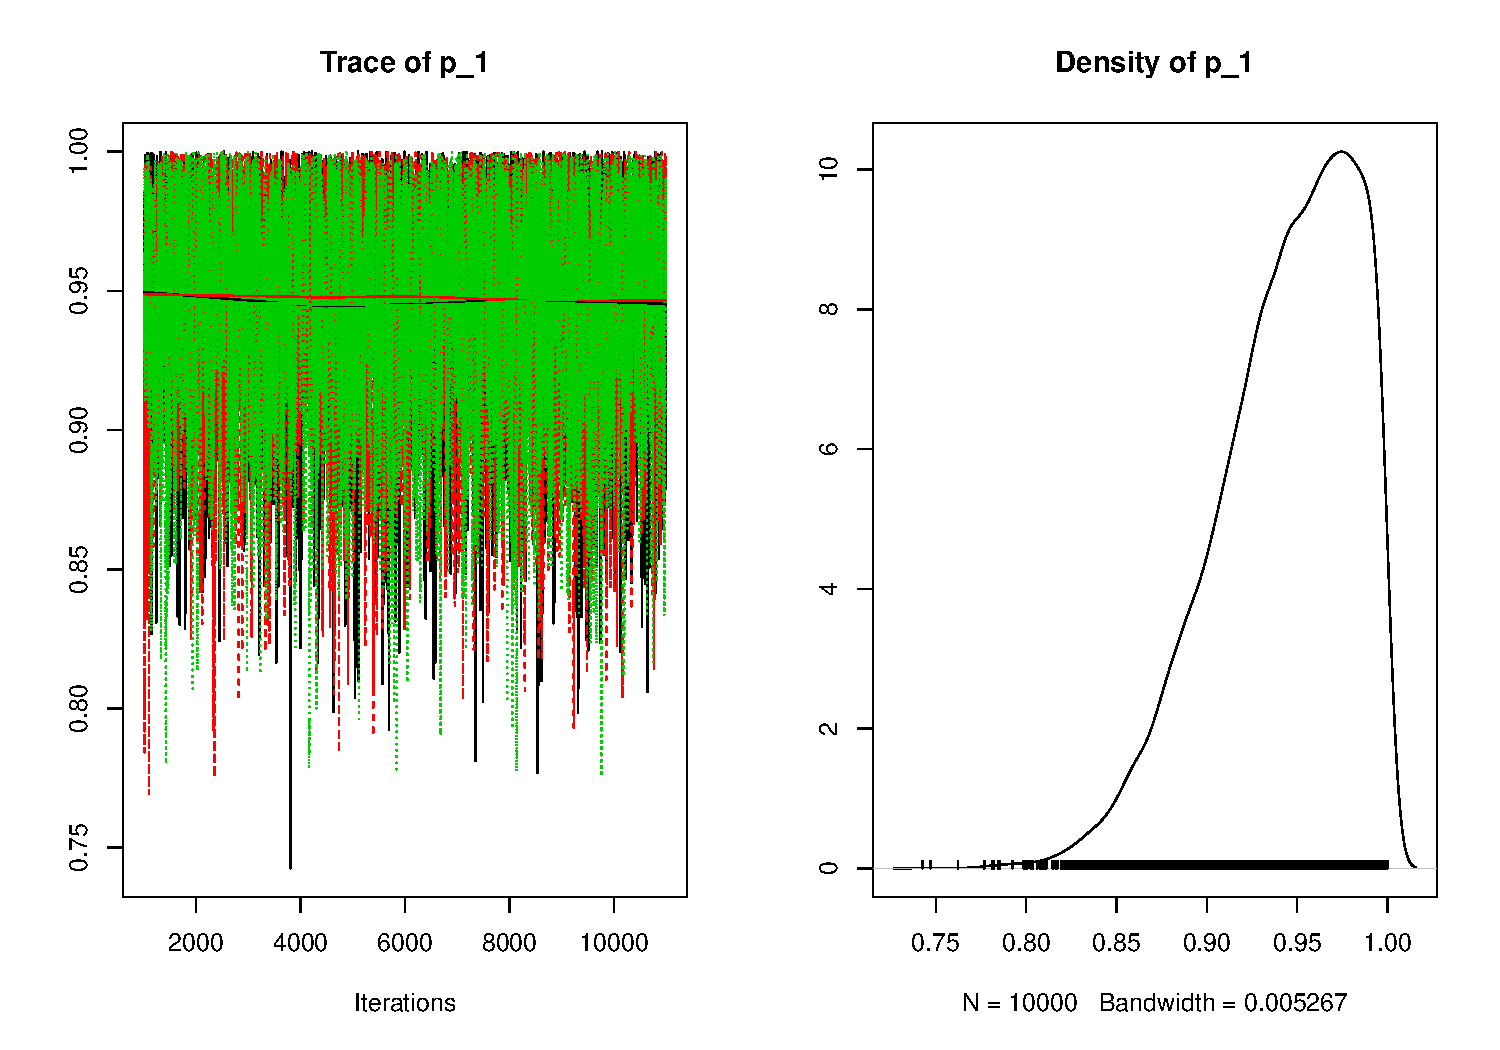
\includegraphics{reg_and_simms_files/figure-beamer/unnamed-chunk-17-1} \end{center}
\end{frame}

\begin{frame}[fragile]{Convergence checking 3}
\protect\hypertarget{convergence-checking-3}{}
\begin{itemize}
\tightlist
\item
  The different colours show the three chains. The location and
  variability should be broadly the same between chains
\item
  There are some useful statistical tests for convergence, including the
  \emph{Geweke} test which looks to see whether the mean is stable in
  each half of the iterations, or the \emph{Brooks, Gelman, Rubin} (BGR)
  test which looks to see whether different chains match.
\item
  Both \texttt{simmr} and \texttt{MixSIAR} use the BGR test
\item
  The BGR test is best if you have multiple chains
\end{itemize}
\end{frame}

\begin{frame}[fragile]{Convergence checking 4}
\protect\hypertarget{convergence-checking-4}{}
\begin{itemize}
\tightlist
\item
  If you started by choosing bad initial values you might want to remove
  an initial chunk of the samples. This is known as the burn in and can
  be set using the \texttt{n.thin} command in the \texttt{jags} function
  call
\item
  Ideally the samples from the posterior distribution should be
  independent. If the algorithm isn't working well you can \emph{thin}
  them out with the \texttt{n.thin} argument in the \texttt{jags}
  function. The auto-correlation plot produced by \texttt{acf} in
  \texttt{R} can tell you whether you need to thin or not
\item
  Finally, we need to choose the number of iterations. For very simple
  models 1,000 is usually fine, but for very complicated models you can
  sometimes need hundreds of thousands or millions. 10,000 is usually a
  good number for most problems. You can set the number of iterations in
  JAGS with \texttt{n.iter}
\end{itemize}

\texttt{simmr}/\texttt{MixSIAR} have their own commands for dealing with
burn-in/thinning/iterations
\end{frame}

\begin{frame}{Summary}
\protect\hypertarget{summary}{}
\begin{itemize}
\tightlist
\item
  A SIMM is very similar to a linear regression. Things get slightly
  more complicated when we move to multiple isotopes
\item
  The priors for a SIMM involve distributions for the source values, the
  dietary proportions, and the residual standard deviation
\item
  When running a Bayesian model, remember to check your model (if
  possible) using posterior predictive checks, and convergence checking
\end{itemize}
\end{frame}

\end{document}
